% A LaTeX (non-official) template for ISAE projects reports
% Copyright (C) 2014 Damien Roque
% Version: 0.2
% Author: Damien Roque <damien.roque_AT_isae.fr>

\documentclass[a4paper,12pt]{book}
\usepackage{tabto}
\usepackage{microtype}
\usepackage[utf8]{inputenc}
\usepackage[utf8]{vietnam}
\usepackage{algorithm}
\usepackage{algpseudocode}
\usepackage{pseudocode}
\usepackage{enumerate}
%\usepackage[T1]{fontenc}
%\usepackage[frenchb]{babel} % If you write in French
%\usepackage[english]{babel} % If you write in English
\usepackage[vietnamese]{babel}
\usepackage{a4wide}
\usepackage{graphicx}
\graphicspath{{images/}}
\usepackage{subfig}
\usepackage{tikz}
\usetikzlibrary{shapes,arrows}
\usepackage{pgfplots}
\pgfplotsset{compat=newest}
\pgfplotsset{plot coordinates/math parser=false}
\newlength\figureheight
\newlength\figurewidth
\pgfkeys{/pgf/number format/.cd,
set decimal separator={,\!},
1000 sep={\,},
}
\usepackage{ifthen}
\usepackage{ifpdf}
\ifpdf
\usepackage[pdftex]{hyperref}
\else
\usepackage{hyperref}
\fi
\usepackage{color}
\hypersetup{%
colorlinks=true,
linkcolor=black,
citecolor=black,
urlcolor=black}

\renewcommand{\baselinestretch}{1.05}
\usepackage{fancyhdr}
\pagestyle{fancy}
\fancyfoot{}
\fancyhead[LE,RO]{\bfseries\thepage}
\fancyhead[RE]{\bfseries\nouppercase{\leftmark}}
\fancyhead[LO]{\bfseries\nouppercase{\rightmark}}
\setlength{\headheight}{15pt}

\let\headruleORIG\headrule
\renewcommand{\headrule}{\color{black} \headruleORIG}
\renewcommand{\headrulewidth}{1.0pt}
\usepackage{colortbl}
\arrayrulecolor{black}

\fancypagestyle{plain}{
  \fancyhead{}
  \fancyfoot[C]{\thepage}
  \renewcommand{\headrulewidth}{0pt}
}

\makeatletter
\def\@textbottom{\vskip \z@ \@plus 1pt}
\let\@texttop\relax
\makeatother

\makeatletter
\def\cleardoublepage{\clearpage\if@twoside \ifodd\c@page\else%
  \hbox{}%
  \thispagestyle{empty}%
  \newpage%
  \if@twocolumn\hbox{}\newpage\fi\fi\fi}
\makeatother

\usepackage{amsthm}
\usepackage{amssymb,amsmath,bbm}
\usepackage{array}
\usepackage{bm}
\usepackage{multirow}
\usepackage[footnote]{acronym}

\newcommand*{\SET}[1]  {\ensuremath{\mathbf{#1}}}
\newcommand*{\VEC}[1]  {\ensuremath{\boldsymbol{#1}}}
\newcommand*{\FAM}[1]  {\ensuremath{\boldsymbol{#1}}}
\newcommand*{\MAT}[1]  {\ensuremath{\boldsymbol{#1}}}
\newcommand*{\OP}[1]  {\ensuremath{\mathrm{#1}}}
\newcommand*{\NORM}[1]  {\ensuremath{\left\|#1\right\|}}
\newcommand*{\DPR}[2]  {\ensuremath{\left \langle #1,#2 \right \rangle}}
\newcommand*{\calbf}[1]  {\ensuremath{\boldsymbol{\mathcal{#1}}}}
\newcommand*{\shift}[1]  {\ensuremath{\boldsymbol{#1}}}

\newcommand{\eqdef}{\stackrel{\mathrm{def}}{=}}
\newcommand{\argmax}{\operatornamewithlimits{argmax}}
\newcommand{\argmin}{\operatornamewithlimits{argmin}}
\newcommand{\ud}{\, \mathrm{d}}
\newcommand{\vect}{\text{Vect}}
\newcommand{\sinc}{\ensuremath{\mathrm{sinc}}}
\newcommand{\esp}{\ensuremath{\mathbb{E}}}
\newcommand{\hilbert}{\ensuremath{\mathcal{H}}}
\newcommand{\fourier}{\ensuremath{\mathcal{F}}}
\newcommand{\sgn}{\text{sgn}}
\newcommand{\intTT}{\int_{-T}^{T}}
\newcommand{\intT}{\int_{-\frac{T}{2}}^{\frac{T}{2}}}
\newcommand{\intinf}{\int_{-\infty}^{+\infty}}
\newcommand{\Sh}{\ensuremath{\boldsymbol{S}}}
\newcommand{\C}{\SET{C}}
\newcommand{\R}{\SET{R}}
\newcommand{\Z}{\SET{Z}}
\newcommand{\N}{\SET{N}}
\newcommand{\K}{\SET{K}}
\newcommand{\reel}{\mathcal{R}}
\newcommand{\imag}{\mathcal{I}}
\newcommand{\cmnr}{c_{m,n}^\reel}
\newcommand{\cmni}{c_{m,n}^\imag}
\newcommand{\cnr}{c_{n}^\reel}
\newcommand{\cni}{c_{n}^\imag}
\newcommand{\tproto}{g}
\newcommand{\rproto}{\check{g}}
\newcommand{\LR}{\mathcal{L}_2(\SET{R})}
\newcommand{\LZ}{\ell_2(\SET{Z})}
\newcommand{\LZI}[1]{\ell_2(\SET{#1})}
\newcommand{\LZZ}{\ell_2(\SET{Z}^2)}
\newcommand{\diag}{\operatorname{diag}}
\newcommand{\noise}{z}
\newcommand{\Noise}{Z}
\newcommand{\filtnoise}{\zeta}
\newcommand{\tp}{g}
\newcommand{\rp}{\check{g}}
\newcommand{\TP}{G}
\newcommand{\RP}{\check{G}}
\newcommand{\dmin}{d_{\mathrm{min}}}
\newcommand{\Dmin}{D_{\mathrm{min}}}
\newcommand{\Image}{\ensuremath{\text{Im}}}
\newcommand{\Span}{\ensuremath{\text{Span}}}

\newtheoremstyle{break}
  {11pt}{11pt}%
  {\itshape}{}%
  {\bfseries}{}%
  {\newline}{}%
\theoremstyle{break}

%\theoremstyle{definition}
\newtheorem{definition}{Définition}[chapter]

%\theoremstyle{definition}
\newtheorem{theoreme}{Théorème}[chapter]

%\theoremstyle{remark}
\newtheorem{remarque}{Remarque}[chapter]

%\theoremstyle{plain}
\newtheorem{propriete}{Propriété}[chapter]
\newtheorem{exemple}{Exemple}[chapter]

\parskip=5pt
%\sloppy

\begin{document}

%%%%%%%%%%%%%%%%%%
%%% First page %%%
%%%%%%%%%%%%%%%%%%

\begin{titlepage}
\begin{center}


\includegraphics[width=0.2\textwidth]{bk}\\[1cm]

{\large Đại học bách khoa Hà Nội}\\[0.5cm]

{\large Khoa học máy tính}\\[0.5cm]

% Title
\rule{\linewidth}{0.5mm} \\[0.4cm]
{ \huge \bfseries Đánh giá độ chính xác của phương pháp lọc cộng tác trong hệ khuyến nghị áp dụng cho bộ dữ liệu movielen \\[0.4cm] }
\rule{\linewidth}{0.5mm} \\[1.5cm]

% Author and supervisor
\noindent
\begin{minipage}{0.4\textwidth}
  \begin{flushleft} \large
    \emph{Sinh viên thực hiện :}\\
    Phạm Văn Cường \\
    Đàm Văn Tài
  \end{flushleft}
\end{minipage}%
\begin{minipage}{0.4\textwidth}
  \begin{flushleft} \large
    \emph{Giảng viên hướng dẫn :} \\
    Ms. Trần Vĩnh Đức \\
    Ms. Trịnh Anh Phúc \\
    Ms. Đinh Viêt Sang
  \end{flushleft}
\end{minipage}

\vfill

% Bottom of the page
{\today}

\end{center}
\end{titlepage}

%%%%%%%%%%%%%%%%%%%%%%%%%%%%%
%%% Non-significant pages %%%
%%%%%%%%%%%%%%%%%%%%%%%%%%%%%

\frontmatter

\chapter*{Tóm tắt}
Hệ khuyến nghị là một công nghệ đang được sử dụng rộng rãi bởi các trang web thương mại điện tử và một vài dịch vụ trưc tuyến khác, để dự đoán ý kiến người sử dụng về sản phẩm. Báo cáo này giới thiệu về hai thuật toán khuyến nghị đặc biệt là FunkSVD, thuật toán nhân tử ma trận và lọc cộng tác dựa trên sản phẩm, cái mà sử dụng độ tương đồng giữa hai sản phẩm. Mục tiêu là để so sánh đô chính xác dự đoán của các thuật toán khi chạy trên bộ dữ liệu nhỏ và lớn. Bằng việc thực hiện đánh giá chéo trong các thuật toán

\clearpage
\tableofcontents

\clearpage
\listoffigures

\clearpage
\listoftables
%\clearpage
%\chapter*{Liste des sigles et acronymes}
%\begin{acronym}[CP-OFDMX] % Give the longest acronym here
%\acro{ASK}{\emph{Amplitude Shift Keying}}
%\acro{AWGN}{\emph{Additive White Gaussian Noise}}
%\acro{BABG}{Bruit Additif Blanc Gaussien}
%\acro{BCJR}{\emph{Bahl, Cocke, Jelinek, Raviv}}
%\acro{BER}{\emph{Binary Error Rate}}
%\acro{BFDM}{\emph{Biorthogonal Frequency Division Multiplexing}}
%\end{acronym}

%%%%%%%%%%%%%%%%%%%%%%%%%%%%%%%%%%%%%%%%%%%%
%%% Content of the report and references %%%
%%%%%%%%%%%%%%%%%%%%%%%%%%%%%%%%%%%%%%%%%%%%

\mainmatter
\pagestyle{fancy}

\cleardoublepage

\chapter*{Giới thiệu}
\addcontentsline{toc}{chapter}{Giới thiệu}
\markboth{Giới thiệu}{Giới thiệu}
\label{chap:Giới thiệu}
%\minitoc

Hệ khuyến nghị là một công nghệ dựa trên một hệ thống học cung cấp dự đoán đến người sử dụng của một dịch vụ web hoặc ứng dụng, dựa trên hành vi người sử dụng. Nghiên cứu hệ khuyến nghị là một hệ quả của việc kinh doanh, để từ đó nâng cao doanh số bán hàng, thỏa mãn nhu cầu khách hàng. 

Cải thiện vẫn là một vấn đề quan trọng cho các nhà phát triển của hệ khuyến nghị. Hiệu năng thực hiện, độ chính xác là là vấn đề cần cải tiến. 

Báo cáo sẽ tính toán và so sánh độ chính xác trên hai tập dữ liệu movielens.
%%% Local Variables: 
%%% mode: latex
%%% TeX-master: "isae-report-template"
%%% End: 

\chapter{Kiến thức cơ sở}
Chương này sẽ giới thiệu nét chính về khái niệm hệ khuyến nghị, mô tả một vài phương pháp khác nhau và ưu nhược điểm của các phương pháp đó. Phạm vi của báo cáo nằm trong lọc cộng tác

\section{Hệ khuyến nghị}
Mục tiêu chính của hệ khuyến nghị là đánh giá for các mặt hàng và cung cấp một danh sách các mặt hàng được đề nghị cho người mua hàng. Có nhiều phương pháp khác nhau cho nhiệm vụ này, như so sánh các đánh giá, mặt hàng, đặc trưng người mua.

Mọi hệ khuyến nghị cơ bản chứa đựng các thông tin căn bản như: tập người mua hàng, tập các mặt hàng và quan hệ giữa chúng (các đánh giá của người mua cho từng mặt hàng). Đánh giá cho một mặt hàng thường biểu diễn bằng một số nguyên, ví dụ có thể trong khoảng 0 - 5.

Các liên kết cho các thực thể (người mua - mặt hàng) được mô tả bằng đồ thị hai phía. và ma trận. Một công cụ thường sử dụng của hệ khuyến nghị là thông tin người mua và thuộc tính mặt hàng. Thông tin người mua có thể bao gồm nhiều đặc trưng, như: tuổi, giới tính và nghề nghiệp. Thuộc tính của một mặt hàng phụ thuộc nội dung của chúng. Như phim có thể có các đặc trưng về thể loại, danh sách diễn viên.

Hệ khuyến nghị có thể phân loại đến ba thể loại chính:
\begin{enumerate}[1.]
	\item \textbf{Lọc dựa trên nội dung (Content-based filtering):} Khuyến nghị các mặt hàng giống về nội dung với các mặt hàng khác được người mua đã đánh giá tốt.
	\item \textbf{Lọc cộng tác (Collaborative filtering):} khuyến nghị các mặt hàng bằng việc so sánh độ tương đồng của hai người mua dựa vào bảng đánh giá các sản phẩm mà họ mua từ đó tìm ra tập người mua tương đồng với nhau. Sau đó sẽ đánh giá các mặt hàng mà người mua chưa đánh giá (đây gọi là lọc cộng tác dựa trên user-user). Hệ thống lọc cộng tác có thể chia ra làm hai phương pháp là dựa trên bộ nhớ (memory-based) và  dựa trên mô hình.
	\item \textbf{Lọc kết hợp (Hybrid filtering):} khuyến nghị mặt hàng bằng việc tổ hợp hai hệ thống lọc trên.
\end{enumerate}

\section{Hệ thống dựa theo nội dung (Content-based)}
Trong hệ thống dựa theo nội dung, một khuyến nghị được dựa trên liên kết giữa các thuộc tính của các mặt hàng đã được người mua đánh gía và chưa đánh giá. Phương pháp này sử dụng khái niệm nhất quán sự quan tâm của mỗi cá nhân, sẽ không thay đổi trong tương lại gần.

Giả sử mỗi người mua đã đánh giá một tập mặt hàng, từ đó ta có thể xây dụng bảng thông tin cá nhân của người đó dựa trên các đặc trưng nội dung của mặt hàng để từ đó xác định các mặt hàng khác có các đặc trưng nằm trong bảng thông tin đó.

\section{Hệ thống lọc cộng tác (Collaborative filtering)}
Hệ thống lọc cộng tác khuyến nghị các mặt hàng đến người sử dụng bởi so sánh đánh giá của người sử dụng. Ý kiến của người mua trong thực tế đóng vai trò quan trọng cho việc ra quyết định mua hay không mua. Hệ thống sẽ tìm ra những người dùng có những đánh giá tương đồng.

\begin{table}[H]
\caption{Đánh gía user-item. Đánh giá trong khoảng 1-5, 5 là tốt nhất và 1 là tệ nhất}
\label{table:1}
\begin{center}
\begin{tabular}{|c|c|c|c|c|}
\hline 
Rating Matrix & The Avengers & The Revevant & The Martian & Deadpool \\ 
\hline 
Fred & 2 & 4 & 5 & 1 \\ 
\hline 
Sara & ? & 5 & ? & 2 \\ 
\hline 
John & 5 & 2 & 2 & 4 \\ 
\hline 
Jessica & ? & 1 & ? & 5 \\ 
\hline 
\end{tabular} 
\end{center}
\end{table}

Table \ref{table:1} là một ví dụ về hoạt động của hệ lọc công tác khuyến nghị một mặt hàng sử dụng thông tin từ các người sử dụng khác. Đánh giá user-item có thể được nhìn như một ma trận, như biểu diễn trong bảng. Mỗi hàng trong bảng \ref{table:1} biểu diễn một người sử dụng và mỗi cột   một phim, đánh giá nằm trong khoảng 1-5.

Để cung cấp để xuất cho người mua, hệ thống xác định những người dùng khác dựa trên thông tin các mẫu được đánh giá bởi họ. Các mặt hàng được đề xuất sẽ dựa theo nhưng người tương đồng với người đó. Với một lượng lớn người mua đánh giá trong một hệ thống thực, sẽ cho nhiều độ chính xác hơn.

Một nhược điểm của thuật toán cộng tác là đề nghị hệ thống có nhiều đánh giá cho các mặt hàng để đặt được độ chính xác khi đề xuất.

\section{Hệ thống kết hợp (Hybrid Approaches)}
Để cố gắng đạt được nhiều đề xuất chính xác, phương pháp kết hợp được đề xuất. Một thuật toán kết hợp là tổ hợp của nhiều phương pháp nhằm đạt được kết quả chính xác. Ý tưởng chung đằng sau của phương pháp kết hợp được mô tả dưới đây:
\begin{enumerate}[1.]
	\item Một hệ thống kết hợp có thể dự đoán đề xuất từ một tập dữ liệu, sử dụng cả một phương pháp dựa trên nội dung và phương pháp lọc. Khi dự đoán này được sử dụng, một số liệu cụ thể có thể được sử dụng để xác định độ chính xác của các khuyến nghị, để xác định tập đề xuất. Ngoài ra, kết quả có thể được kết hợp để tạo ra kết quả đề xuất cao nhất từ cả hai cách tiếp cận.
	\item Một hệ thống kết hợp có thể dự đoán đề xuất từ một tập dữ liệu sử dụng phương pháp lọc cộng tác kết hợp chặt chẽ với một vài nôi dung đặc trưng của phương pháp dựa trên nội dung.
	\item Một hệ thống kết hợp có thể dự đoán đề xuất từ một tập dữ liệu sử dụng phương pháp dựa trên nội dung kết hợp với một vài đặc tả của phương pháp cộng tác.
\end{enumerate}

\section{Thuật toán dựa trên bộ nhớ (Memory-based Algorithms)}
Thuật toán dựa trên bộ nhớ sử dụng lý thuyết xác suất để tìm tập mua,  thường được gọi là hàng xóm, đó là những người mua tương tự. Một hàng xóm tìm bởi lọc cộng tác được thực hiện tính toán độ tương đồng. Độ tương đồng được tính bằng tương quan khoảng cách giữa những người mua, và những mặt hàng. Một sản phẩm dự đoán đến người mua được sinh ra bằng tính toán  trung bình đánh giá của người mua tương đồng đối với sản phẩm đó. Hệ thống này được sử dụng trong thương mại điện tử điển hình là trang web Amazon.com 

Tuy nhiên thuật này cũng có vài giới hạn, đặc biệt khi tập dữ liệu thưa, để tìm người mua tương đồng là rất khó khăn và không chính xác.

\section{Thuật toán dựa trên mô hình (Model-based Algorithm)}
Thuật toán dựa trên mô hình khác với dựa trên bộ nhớ bởi sử dụng thuật toán học máy, thuật toán khai phá dữ liệu hoặc một thuật toán khác để tìm kiểu mẫu đặc trưng và dự đoán đánh giá bằng việc học. Một vài phương pháp cho dựa thuật toán dựa trên mô hình là mô hình phân cụm, mô hình bayesian va các mô hình phụ thuộc.

\section{Các vấn đề}
Ngày nay, hệ khuyến nghị đối mặt với nhiều vấn đề, bao gồm thực thi, thuộc tính người sử dụng và vấn đề về hiệu năng. Thêm vào đó, các thuộc tính của tập dữ liệu cũng là một thử thách.
\subsection{Thực thi}
Hệ khuyến nghị đối mặt với nhiều thử thách, các thuật toán thường có các nhược điểm riêng của chúng. Mặc dù một số phương pháp tiếp cận có hiệu quả về thời gian và đưa ra dự đoán chính xác nhưng kết quả lại đem đến kết quả không chính xác. Lý do về dữ liệu ít cũng làm giảm độ chính xác.
\subsection{Hiệu năng}
Sự phát triển nhanh của cơ sở dữ liệu bao gồm user-item có thể dẫn đến vấn đề về hiệu năng. Dịch vụ bao gồm hàng triệu mặt hàng và người mua đem lại độ chính xác cho hệ khuyến nghị nhưng mặt khác tính toán như vậy có thể quá chậm.
\subsection{Thuộc tính người mua}
Khó để đánh giá, mức độ thuộc tính của người mua đối với các mặt hàng một cách chính xác cụ thể. Vấn đề về đánh giá không chính xác của người mua về mặt hàng và số lượng đánh giá quá ít, không thể làm nổi bật được đặc điểm của người mua.
\subsection{Tập dữ liệu}
Tập dữ liệu được sử dụng để đánh giá thuật toán có tác động lớn tới kết quả. Khi đánh giá một thuật toán. Chọn bộ dữ liệu phù hợp các thuộc tính độc lập. Các thuộc tính của tập dữ liệu có ảnh hưởng tới thuật toán. ví dụ:
\begin{enumerate}[1.]
	\item Mật độ của tập dữ liệu.
	\item Tỉ lệ giữa người mua và mặt hàng (user-item)
\end{enumerate}
Mật độ là quan trọng vì người mua chỉ đánh giá một tập con nhỏ tất cả các mặt hàng. Tập dữ liệu thưa thường cho kết quả dự đoán không chính xác.
\section{Đánh giá}
Hiệu năng thuật toán khuyến nghị có thể được đo bằng cách kiểm tra lại trên các tập dữ liệu khác nhau. Trong báo cáo này, đánh giá chéo được sử dụng để kiểm tra hiệu năng của thuật toán dự đoán. Hiệu năng của thuật toán dự đoán được đo với nhiều công thức khác nhau. Công thức được sử dụng phụ thuộc và mục đích của thuật toán và mục tiêu của phép đo.
\subsection{Trung bình trị tuyệt đối của lỗi (Mean Absolute Error}
Mean absolute error(MAE) là công thức được sử dụng để tính trung bình của tất cả giá trị tuyệt đối khác nhau giữa đánh giá dự đoán và đánh giá đúng. MAE thấp cho độ chính xác cao. Tổng quan MAE có thể từ 0 cho đến vô hạn, khi vô hạn là lỗi lớn nhất. Công thức của MAE 
\begin{center}
MAE = $ \frac{1}{n}\sum^{n}_{i=1}|ratingactual_{i}| - |ratingpredicted_{i}|$
\end{center}
n is the amount of ratings
\\ rating\- actual is the actual rating
\\ rating\- predicted is predicted rating
\subsection{Căn bậc hai trung bình của bình phương lỗi}
Root mean square error(RMSE) tính giá trị trung bình của tất cả bình phương hiệu giữa đánh giá đúng và đánh giá dự đoán và sau đó tính căn bậc hai để ra kết quả. Công thức của RMSE:
\begin{center}
$RMSE = \sqrt{\frac{1}{n}\sum^{n}_{i=1}(ratingactual_{i} - ratingpredicted_{i})^2}$
\end{center}
n is the amount of ratings
\\ rating\- actual is the actual rating
\\ rating\- predicted is predicted rating

\subsection{Đánh giá chéo}
Đánh giá chéo được hiểu như là đánh giá xoay vòng, ta chia dữ liệu thành các n bộ sau chọn n-1 bộ để làm tập dữ liệu đào tạo và tập còn lại để đánh giá, cứ làm như vậy cho đến khi mọi tập đều được chọn làm đánh giá. Kết quả cuối cùng sẽ là giá trị trung bình của mỗi lần chọn.
%ua%% Local Variables: 
%%% mode: latex
%%% TeX-master: "isauae-report-template"
%%% End: 
\chapter{Thuật toán}
\section{Lọc cộng tác dựa trên mặt hàng (Item-based Collaborative Filtering)}
Phương pháp lọc cộng tác dựa trên mặt hàng so sánh người mua và đánh giá của họ đối với một tập mặt hàng nhất định. Thuật toán tính toán hàng xóm gần nhất của người mua. Mọi hàng xóm trước đã đánh giá mặt hàng được so sánh đến mặt hàng với độ tương đồng giữa các mặt hàng. Khi đa số các mặt hàng tương tự đã xác định. Sự dự đoán được tính toán bởi trung bình trọng số của các đánh giá của hàng xóm và độ tương tự của người đó và hàng xóm. Tính toán độ tương đồng của mặt hàng đã được làm với một vài phương thức bao gồm độ tương tự dựa trên cosine, độ tương tự đựa phép tương quan và độ tương đồng cosine điều chỉnh.
\subsection{Độ tương tự dựa trên Cosine (Cosine-based Similarity}
Cosine-based similarity là một phương pháp tính toán độ tương tự giữa các mặt hàng trong phương pháp lọc cộng tác dựa trên mặt hàng. Trong phương pháp này, một mặt hàng được biểu diễn giống một vector trong không gian người sử dụng. Góc giữa hai vector được tính và cosine của góc là độ tương tự của các mặt hàng. Cho ví dụ hai mặt hàng m và n được tính như sau:
\begin{center}
$similarities(m, n) = cosine(\bar{m},\bar{n}) = \frac{\bar{m}*\bar{n}}{||\bar{m}||_{2}*||\bar{n}||_{2}}$
\end{center}
Toán tử \" * \" biểu thị toán tử nhân giữa hai vector.

Tính toán độ tương tự dựa trên cosine có một khó khăn. Tỉ lệ đáng giá của người mua không được cân nhắc trong lúc tính toán. Tính toán được thực hiện qua thông tin từ một vài cột, và mỗi cột đại diện cho một người sử dụng khác. Vấn đề này có thể giải quyết với độ tương tự cosine điều chỉnh bằng cách trừ đi trung bình đánh giá của người mua đó ở mỗi cột đã đánh giá. Độ tương đồng của hai mặt hàng m và n, sử dụng độ tương tự cosine điều chỉnh là:
\begin{center}
$similarity(m, n) = \frac{\sum_{u\in U}(R_{u,m}-\bar{R}_{u})(R_{u,n}-\bar{R}_{u})}{\sqrt{(R_{u,m} - \bar{R}_u)^{2}} \sqrt{(R_{u,n} - \bar{R}_u)^{2}}}$
\end{center}
$R_{u,m}$ là đánh giá của người sử dụng u cho mặt hàng m.
$\bar{R}_{u}$ là đánh giá trung bình cho người mua u.

\subsection{Độ tương tự dựa trên tương quan {Correlation-based Similarity}}

Độ tương tự dựa trên tương quan giữa hai mặt hàng m và n được tính bằng tương quan Pearson. Độ tương quan Pearson cho mặt hàng m và n được đánh giá bởi một tập người sử dụng U được tính toán như sau:
\begin{center}
$similarity(m, n) = \frac{\sum_{u\in U}(R_{u,m}-\bar{R}_{m})(R_{u,n}-\bar{R}_{n})}{\sqrt{(R_{u,m} - \bar{R}_m)^{2}} \sqrt{(R_{u,n} - \bar{R}_n)^{2}}}$
\end{center}
$\bar{R}_{u}$ là trung bình đáng giá của người sử dụng u.
%%% Local Variables: 
%%% mode: latex
%%% TeX-master: "isae-report-template"
%%% End:
\subsection{Tính toán dự đoán} 
Tính toán dự đoán đạt được bởi một vài công nghệ. Một phương pháp đơn giản là tính toán tổng trọng số của một mặt hàng m cho người mua u bằng lấy tổng của tất cả đánh giá các mặt hàng của người mua u tương đồng với m. Mục đích của phương pháp này là để hiểu đánh giá của một người mua cho các mặt hàng mà tương đồng đến mặt hàng đó là một phương pháp thử để dự đoán các đánh giá. Tổng trọng số cho dự đoán một mặt hàng m của người mua u được tính như sau:
\begin{center}
$P_{u, m} = \frac{(\sum_{N}(s_{m,k}*R_{u,k})}{\sum_{N}(|s_{m,k}|)}$
\end{center}
$P_{u, m}$ là dự đoán đánh giá của mặt hàng m của người mua u 
$R_{u, k}$ là đánh giá của người mua u cho mặt hàng k
N là tập các mặt hàng tương tự với m
k là một phần tử của N
$s_{m, k}$ là độ tương tự của hai item m và k.

\section{FunkSVD}
FunkSVD là một thuật toán sử dụng phương pháp tìm thừa số ma trận, tên là phân tích giá trị riêng (SVD). Phân tích giá trị riêng được sử dụng để giảm một ma trận đến hai ma trận với số chiều ít hơn. Hai ma trận kết quả được sinh ra biểu diễn các mặt hàng và người mua. Dự đoán được tính bằng tích của một hoặc nhiều vector mặt hàng và một vector người sử dụng. Một ví dụ của phân tích giá trị riêng giảm một trận đến hai ma trận khác được biểu diễn trong hình dưới. Trong hình, ta thấy u1 to u4 biểu thị các người mua, i1 đến i3 biểu thị các mặt hàng và f1 đến f3 biểu thị tính năng. Các tính năng thường được gọi là nhân tố ẩn
\begin{center}
\begin{figure}[H]
	\centering
	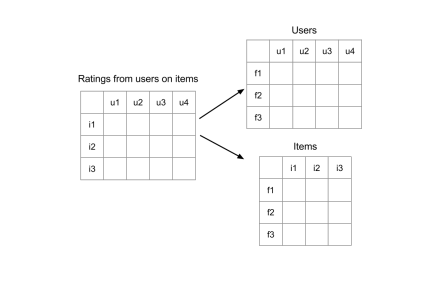
\includegraphics[width=1\textwidth]{svd.png}
	\caption{Singular value decomposition in a dataset}
	\label{fig:SVD}
\end{figure}
\end{center}
FunkSVD đào tạo ra một mô hình để đạt được độ chính xác nhất có thể cho các mặt hàng và người mua. Trong quá trình đào tạo, thuật toán có một tham số được gọi là số vòng lặp. Số vòng lặp thể hiện có bao nhiêu lần đào tạo cho một ô trong ma trận được cho là chạy. Số vòng lặp có thể là một số cố định hoặc tùy theo một số giới hạn khác để kết thúc vòng lặp.

Một ưu điểm của phân tích giá trị riêng là hai ma trận phân tích thường có ước lượng tốt hơn so với ma trận ban đầu. Mục đích của nhân tử ma trận là sinh ra dữ liệu bằng việc trích xuất sở thích người mua phổ biến, phân loại chúng để có được cái nhìn tổng quát của người mua.
\chapter{Kinh nghiệm}
Ta sử dụng ngôn ngử lập trình python và các thư viện cơ bản trong tính toán khoa học trong python.

Về phần hệ khuyến nghị ta sử dụng thư viện graphlab 

Còn phần thực hiện FunkSVD ta sử dụng thư viện pyRecLab (Recommendation lab for Python)
\section{Datasets}
Kiểm tra được thực hiện trong hai tập dữ liệu Movielens được cung cấp bởi GroupLens. Tập dữ liệu Movielens bao gồm đánh giá của người xem cho phim. Hai tập đó có kích thước khác nhau, độc lập với nhau. Tập dữ liệu được sử dụng trong báo cáo là 100k phát hành năm 1988 và 1M được phát hành năm 2003. Cả hai tập dữ liệu bao gồm các người xem đánh giá ít nhất 20 phim. Nó bao gồm 100000 đánh giá từ 943 người xem trong 1682 phim với mật độ 6.37\%. Tham số đưa ra kết quả tốt nhất trong tập Movielens 100k sau đó được đưa vào tập 1M để đánh giá độ chính xác của thuật toán. Tập dữ liệu 1M bao gồm 1 million đánh giá từ 6040 người sử dụng trong 3706 bộ phim với mật độ 4.47\% . Cả hai tập dữ liệu có đánh giá từ 1 đến 5.

Lý do sử dụng hai tập dữ liệu Movielens là bởi vì chúng được sử dụng rãi trong nhiều báo cáo. Họ cũng sử dụng quy ước đánh giá. Cả hai tập dữ liệu là cùng tỉ lệ đánh giá tương ứng. Kích thước hai bộ dữ liệu không quá lớn có thể chạy nhanh ra kết quả.

\begin{table}[H]
\caption{Movielens dataset properties}
\label{table:2}
\begin{center}
\begin{tabular}{|c|c|c|c|c|c|}
\hline 
Name & Users & Movies & Ratings-Scale & Ratings & Density \\ 
\hline 
ML 100k & 943 & 1682 & 1-5 & 100.000 & 6.30\% \\ 
\hline 
ML 1M & 6040 & 3706 & 1-5 & 1.000.209 & 4.47\% \\ 
\hline 
\end{tabular} 
\end{center}
\end{table}

\chapter{Kết quả}
\section{Hệ thống lọc cộng tác dựa trên bộ nhớ}
\begin{table}[H]
\caption{Kết quả hệ thống lọc cộng tác dựa trên bộ nhớ}
\label{table:3}
\begin{center}
\begin{tabular}{|c|c|c|c|c|c|}
\hline 
dataset/error & MAE user & RMSE user & MAE item & RMSE item & RMSE user use correlation \\ 
\hline 
100k & 0.807 & 1.02 & 0.777 & 0.999 \\ 
\hline 
1M \\ 
\hline 
\end{tabular}
\end{center}
\end{table}

\section{Hệ thống lọc dựa trên mô hình}
\subsection{Sử dụng SVD trong tập dữ liệu 100k với các giá trị riêng k khác nhau}
\begin{table}[H]
\caption{Kết quả hệ thống lọc cộng tác dựa trên mô hình sử dụng SVD}
\label{table:4}
\begin{center}
\begin{tabular}{|c|c|c|c|c|c|c|c|c|c|c|}
\hline 
k & 5 & 10 & 15 & 20 & 25 & 30 & 35 & 50 & 70 & 100 \\ 
\hline 
error & 2.82 & 2.76 & 2.76 & 2.78 & 2.81 & 2.85 & 2.88 & 2.98 & 3.1 & 3.24 \\ 
\hline 
\end{tabular}
\end{center}
\end{table}

\begin{center}
\begin{figure}[H]
	\centering
	
\includegraphics[width=1\textwidth]{svd_error.jpg}
	\caption{Error Movielens 100k sử dụng SVD}
	\label{fig:SVD for Movielens 100k}
\end{figure}
\end{center}

\appendix

%\bibliographystyle{authoryear-fr}
%\bibliography{references}

\paragraph{\textbf{Tài liệu tham khảo}}
\begin{enumerate}[1.]
	\item \href{https://cambridgespark.com/content/tutorials/implementing-your-own-recommender-systems-in-Python/index.html}{Implementing your own recommender systems in Python}
	\item \href{https://kth.diva-portal.org/smash/get/diva2:927356/FULLTEXT01.pdf}{Evaluating Prediction Accuracy for Collaborative Filtering Algorithms in Recommender Systems}
	\item \href{http://www.mmds.org/}{Mining of massive datasets}
\end{enumerate}

\clearpage
%%%%%%%%%%%%%%%%
%%% Abstract %%%
%%%%%%%%%%%%%%%%

%\thispagestyle{empty}
%
%\vspace*{\fill}
%\noindent\rule[2pt]{\textwidth}{0.5pt}\\
%{\textbf{Résumé ---}}
%Lorem ipsum dolor sit amet, consectetur adipiscing elit. Sed non risus. Suspendisse lectus tortor, dignissim sit amet, adipiscing nec, ultricies sed, dolor. Cras elementum ultrices diam. Maecenas ligula massa, varius a, semper congue, euismod non, mi. Proin porttitor, orci nec nonummy molestie, enim est eleifend mi, non fermentum diam nisl sit amet erat. Duis semper. Duis arcu massa, scelerisque vitae, consequat in, pretium a, enim. Pellentesque congue. Ut in risus volutpat libero pharetra tempor. Cras vestibulum bibendum augue. Praesent egestas leo in pede. Praesent blandit odio eu enim. Pellentesque sed dui ut augue blandit sodales. Vestibulum ante ipsum primis in faucibus orci luctus et ultrices posuere cubilia Curae; Aliquam nibh. Mauris ac mauris sed pede pellentesque fermentum. Maecenas adipiscing ante non diam sodales hendrerit. Ut velit mauris, egestas sed, gravida nec, ornare ut, mi. Aenean ut orci vel massa suscipit pulvinar. Nulla sollicitudin. Fusce varius, ligula non tempus aliquam, nunc turpis ullamcorper nibh, in tempus sapien eros vitae ligula. Pellentesque rhoncus nunc et augue. Integer id felis.
%
%{\textbf{Mots clés :}}
%Lorem ipsum dolor sit amet, consectetur adipiscing elit. Sed non risus. Suspendisse lectus tortor.
%\\
%\noindent\rule[2pt]{\textwidth}{0.5pt}
%\begin{center}
%  ISAE\\
%  10, avenue Édouard Belin\\
%  BP 54032\\
%  31055 Toulouse CEDEX 4
%\end{center}
%\vspace*{\fill}

\end{document}